\documentclass{beamer}
\usepackage{beamerthemesplit}
\usetheme{SPbGU}
%{CambridgeUS}
% Выпишем часть возможных стилей, некоторые из них могут содержать
% дополнительные опции
% Darmstadt, Ilmenau, CambridgeUS, default, Bergen, Madrid, AnnArbor,Pittsburg, Rochester,
% Antiles, Montpellier, Berkley, Berlin
\usepackage{pdfpages}
\usepackage{amsmath}
\usepackage{cmap} % for serchable pdf's
\usepackage[T2A]{fontenc} 
\usepackage[utf8]{inputenc}
\usepackage[english,russian]{babel}
\usepackage{indentfirst}
\usepackage{amsmath}
\usepackage{dot2texi}
\usepackage{tikz}
\usepackage{fancyvrb}
\usepackage{graphicx}
\usepackage{array}
\usepackage{subcaption}
\usepackage{animate}
\usepackage{multirow}
%\usepackage[usenames,dvipsnames]{color}
\usetikzlibrary{shapes,arrows}
% Если у вас есть логотип вашей кафедры, факультета или университета, то
% его можно включить в презентацию.

%\usefoottemplate{\vbox{}}%  \tinycolouredline{structure!25}% {\color{white}\textbf{\insertshortauthor\hfill% \insertshortinstitute}}% \tinycolouredline{structure}% {\color{white}\textbf{\insertshorttitle}\hfill}% }}

%\logo{\includegraphics[width=1cm]{SPbGU_Logo.png}}

%[GLR-анализатор]
\title[]{Статический анализ динамически формируемых строковых выражений}
%\subtitle[студроект]{Студенческий проект}
\institute[СПбГУ]{
Лаборатория JetBrains на Математико-Механическом факультете \\
Санкт-Петербургского государственного университета }

\author[Григорьев Семён]{Григорьев Семён}

\date{1 апреля 2015г.}

\begin{document}

\begin{frame}
    \begin{tabular}[c c c]{m{2.5cm} m{5.5cm} m{2cm}}
    \begin{center}
        \includegraphics[width=2.5cm]{JBLogoWhite.png}
    \end{center}
    &
    \begin{center}
        
    \end{center}
    &
    \begin{center}
        \includegraphics[width=2cm]{SPbGU_Logo.png}
    \end{center}
    \\
    &&
    \end{tabular}
    \titlepage
\end{frame}

\definecolor{orange}{RGB}{179,36,31}
\begin{frame}[fragile]
	\transwipe[direction=90]
	\frametitle{Встроенные языки}
	\begin{itemize}
		\item Встроенный SQL
		\begin{Verbatim}[commandchars=\\\{\}]
\textcolor{blue}{let} p cond fldLst =
    \textcolor{blue}{let mutable} flds = \textcolor{orange}{"id"}
    \textcolor{blue}{for} fld \textcolor{blue}{in} fldLst \textcolor{blue}{do}
        flds <- flds + \textcolor{orange}{", "} + fld 
    \textcolor{blue}{let} tbl = \textcolor{blue}{if} cond \textcolor{blue}{then} \textcolor{orange}{"table1"} \textcolor{blue}{else} \textcolor{orange}{"table2"}    
    \underline{execute} (\textcolor{orange}{"SELECT"} + flds + \textcolor{orange}{"FROM"} + tbl)
		\end{Verbatim}
		\item JavaScript в Java
		\begin{Verbatim}[commandchars=\\\{\}]
\textcolor{blue}{String} script =
    \textcolor{orange}{"function hello(name) { print(’Hello, ’ + name); }"};
engine.eval(script);
\textcolor{blue}{Invocable} inv = (\textcolor{blue}{Invocable}) engine;
inv.invokeFunction(\textcolor{orange}{"hello"}, \textcolor{orange}{"Scripting!!!"} );
        \end{Verbatim}
	\end{itemize}
\end{frame}

%\begin{frame}[fragile]
%	\transwipe[direction=90]
%	\frametitle{Актуальность}
%	\begin{itemize}
%	    \item Да, новый код так \textbf{\underline{почти}} не пишут. Но:
%        \begin{itemize}
%    	    \item Многое уже написано и оно требует поддержки, сопровождения
%	        \item Альтернатив динамическому SQL пока мало
%	        \item Строковыми выражениями пользуются там, где важна производительность
%	    \end{itemize}
%    \end{itemize}
%\end{frame}

\begin{frame}[fragile]
	\transwipe[direction=90]
	\frametitle{Проблемы}
	\begin{itemize}
	    \item Динамически формируемые выражения --- код на некотором языке и его нужно соответствующим образом поддерживать и обрабатывать
	    \item Однако для стандартных инструментов это просто строки
        \begin{itemize}
    	    \item Ошибки в динамически формируемых выражениях обнаруживаются лишь во время выполнения
	        \item Нет поддержки в IDE
	        \item Затруднён реинжиниринг ПО, разработанного с использованием встроенных языков
	        \item Увеличивается уязвимость систем (SQL-инъекции)
	    \end{itemize}
    \end{itemize}
\end{frame}

\begin{frame}[fragile]
	\transwipe[direction=90]
	\frametitle{Встроенный SQL}
		\begin{Verbatim}[commandchars=\\\{\}]
\textcolor{blue}{let} f () =		
    \textcolor{blue}{let} p cond fldLst =
        \textcolor{blue}{let mutable} flds = \textcolor{orange}{"id"}
        \textcolor{blue}{for} fld \textcolor{blue}{in} fldLst \textcolor{blue}{do}
            flds <- flds + \textcolor{orange}{", "} + fld 
        \textcolor{blue}{let} tbl = \textcolor{blue}{if} cond \textcolor{blue}{then} \textcolor{orange}{"table1"} \textcolor{blue}{else} \textcolor{orange}{"table2"}    
        \underline{execute} (\textcolor{orange}{"SELECT"} + flds + \textcolor{orange}{"FROM"} + tbl)
    p false [\textcolor{orange}{"x"};\textcolor{orange}{"y"}] |> print 
    p true [\textcolor{orange}{"x"};\textcolor{orange}{"z"}] |> print
		\end{Verbatim}
\end{frame}

\begin{frame}[fragile]
	\transwipe[direction=90]
	\frametitle{Вложенность языков}
	\begin{itemize}
	    \item $L_1 = L(f)$ --- язык, задаваемый программой
	    \item $L_2 = L(G)$ --- ``эталонный'' \ язык
	    \item $L_2$ --- КС (почти)
	    \item $L_1$ --- КС ?
	    \item Вопрос: $L_1 \subseteq L_2$ ?
	    \item Разрешим если  $L_1$ --- регулярный, $L_2$ --- детрминированный КС
    \end{itemize}
\end{frame}

%\begin{frame}[fragile]
%	\transwipe[direction=90]
%	\frametitle{Пример работы}
%	\begin{center}
%	    \includegraphics[width=290pt]{picts/Error.png}
%	\end{center}
%\end{frame}

\begin{frame}[fragile]
	\transwipe[direction=90]
	\frametitle{Построение регулярной аппроксимации}
	\begin{itemize}
	    \item $L_1$ --- не регулярный
	    \item Построим $L_R$ --- регулярный: $L_1 \subseteq L_R$
    	\begin{itemize}
    	  \item Такой $L_R$ можно построить: Fang Yu, Muath Alkhalaf, Tevfik Bultan, and Oscar H. Ibarra. 2014. Automata-based symbolic string analysis for vulnerability detection
    	\begin{itemize}
    		\item Учитываются строковые опреации
      \end{itemize}
      \end{itemize}
      \item $L_R = L_1 + L_{\Delta}$
    \end{itemize}
\end{frame}

\begin{frame}[fragile]
	\transwipe[direction=90]
	\frametitle{Лексический анализ}
	\begin{center}
	\begin{tabular}{c|c}
	  Входной граф
	  & Результат токенизации
	  \\
	  \hline
    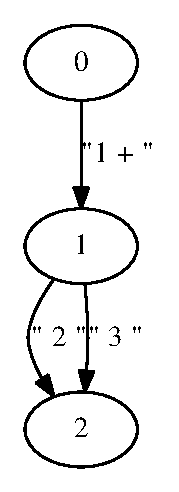
\includegraphics[width=60pt]{picts/before_tokenization.eps}
    & \includegraphics[width=60pt]{picts/after_tokenization.eps}
  \end{tabular}
  \end{center}
\end{frame}

\begin{frame}[fragile]
	\transwipe[direction=90]
	\frametitle{Обобщённый синтаксический анализ}
    \begin{itemize}
    	\item Generalized LR parsing (GLR)
    	\item Предназначен для работы с произвольными КС грамматиками
	    \begin{itemize}
    	    \item Shift-Reduce и Reduce-Reduce конфликты
    	\end{itemize}
    	\item Использует организованный в виде графа стек (GSS)
	   	\item Использует компактное представление леса вывода (SPPF)
	        \begin{itemize}
	            \item Переиспользование общих узлов
	        \end{itemize}
      \item Мы используем RNGLR --- поддерживает произвольные КС грамматики
	\end{itemize}
\end{frame}

\begin{frame}[fragile]
	\transwipe[direction=90]
	\frametitle{Синтаксический анализ строковых выражений}
	\begin{center}
	\begin{tabular}{c|c}
	  Входной граф & Результат разбора
	  \\
	  \includegraphics[width=150pt]{picts/UnambiguousBrackets_Circle.pdf}
	  &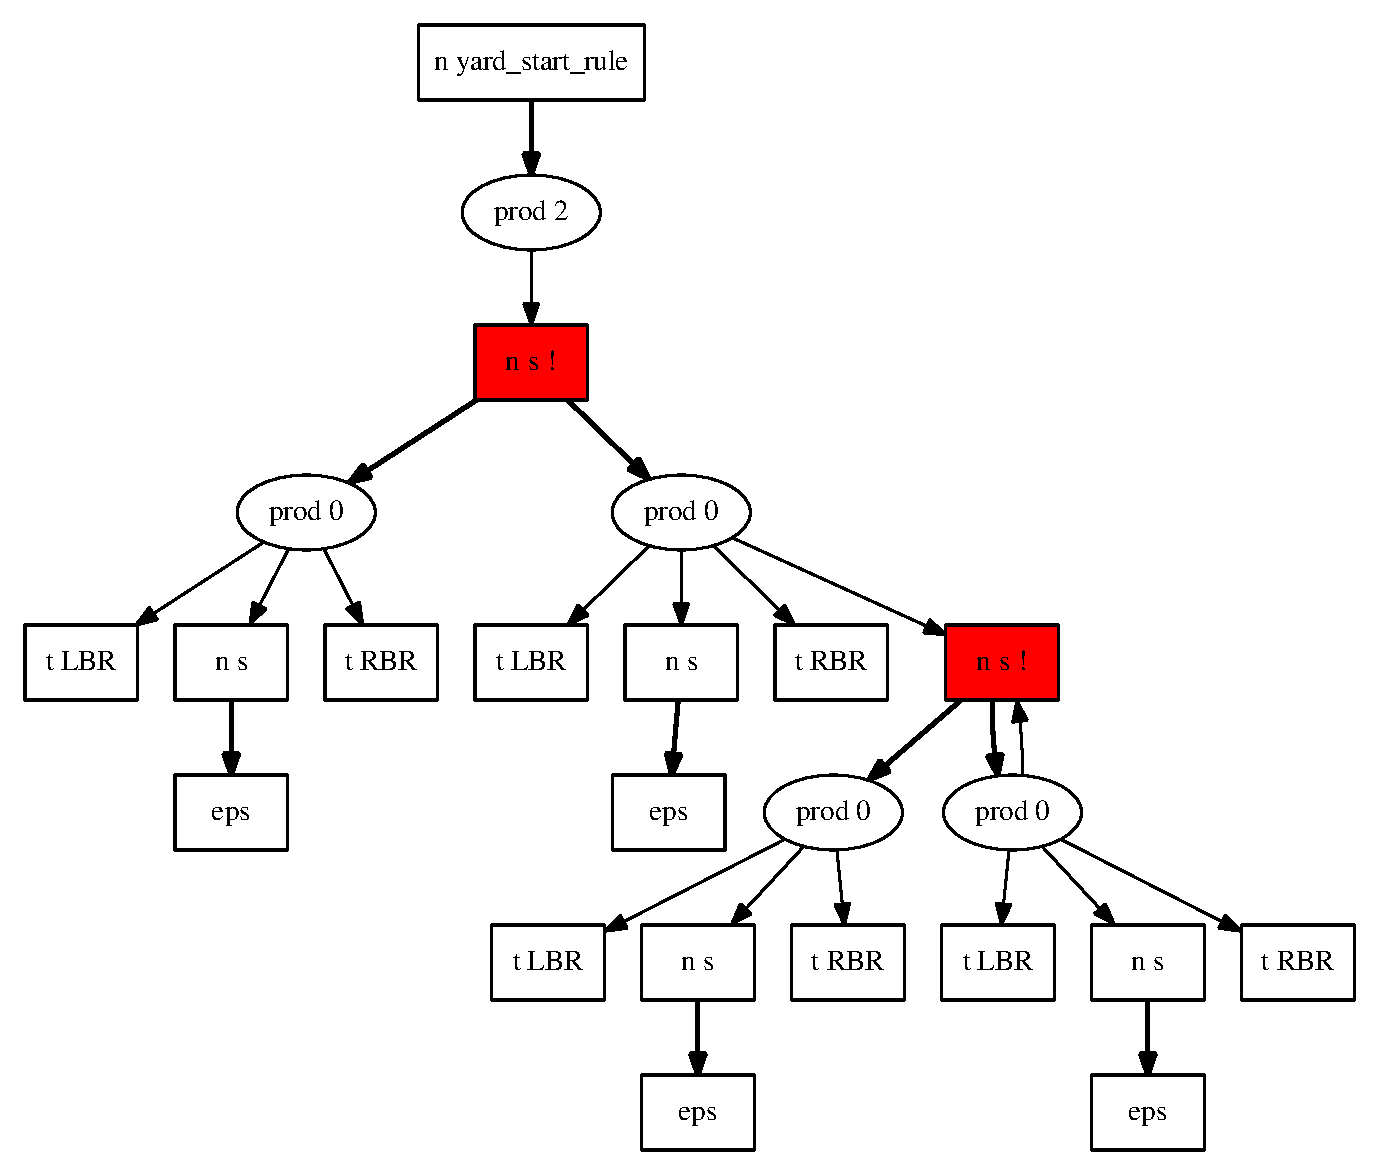
\includegraphics[width=160pt]{picts/sppf.eps}
	    
	  \\
	  Грамматика: 
    $s : LBR \ s \ RBR \ s \ | \ \varepsilon $
  \end{tabular}
  \end{center}
\end{frame}

\begin{frame}[fragile]
	\transwipe[direction=90]
	\frametitle{Синтаксический анализ регулярного множества}
  \begin{itemize}
  \item
	  Входной граф 
	  \\
	  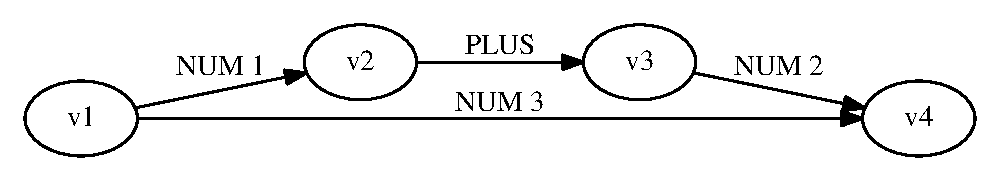
\includegraphics[width=300pt]{picts/agss_input.eps}
	\item
  
	  Грамматика: 
    $expr : NUM \ PLUS \ NUM$
	\item
	  GSS
	  \\
	  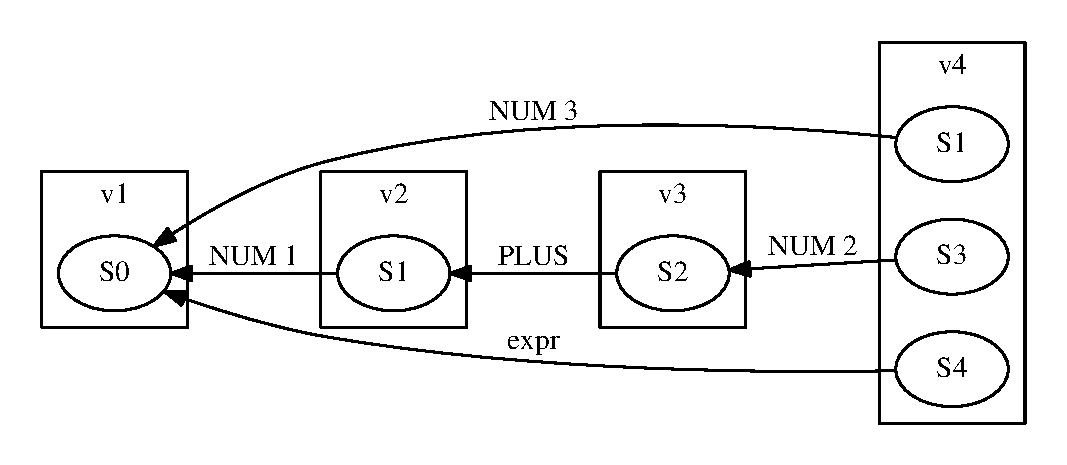
\includegraphics[width=300pt]{picts/agss.eps}
\end{itemize}
\end{frame}


\begin{frame}[fragile]
	\transwipe[direction=90]
	\frametitle{Синтаксический анализ регулярного множества}
  \begin{itemize}
  \item Завершаемость
    \begin{itemize}
      \item Поиск неподвижной точки: для каждой вершины исходного графа вычисляем множество всех возможных LR-состояний
      \item Состояний в каждой вершине не больше чем всего состояний LR-автомата для данной граматики
      \item Все рёбра в GSS уникальны --- не более чем полный граф
    \end{itemize}
\end{itemize}
\end{frame}

\begin{frame}[fragile]
	\transwipe[direction=90]
	\frametitle{Синтаксический анализ регулярного множества}
  \begin{itemize}
  \item Корректность
    \begin{itemize}
      \item Предполагаем, что RNGLR корректен
      \item Ситуации, не попадающие в классический RNGLR --- ``замыкание'' цикла: можем потерять свёртки
      \item Чтобы этого не произошло, нужно запоминать свёртки, в которых участвовало состояние: проходящие свёртки
    \end{itemize}
\end{itemize}
\end{frame}

		   % \animategraphics[autoplay,loop,height=7.5cm]{13}{picts/BigSample/frame_}{001}{334}
		   
\begin{frame}[fragile]
	\transwipe[direction=90]
	\frametitle{Результаты}
	\begin{itemize}
	    \item Предложен алгоритм синтаксического анализа регулярных множеств
	    \begin{itemize}
	        \item Строится структура данных, содержащая деревья вывода всех корректных цепочек анализируемого множества
    	\end{itemize}
    	\item На основе алгоритма реализован генератор синтаксических анализаторов
    	\item Реализован генератор лексических анализаторов для динамически формируемых строковых выражений
      \item Генераторы и набор вспомогательных библиотек объединены в пакет для разработки инструментов статического анализа строковых выражений
	    \item С использованием пакета создан плагин для ReSharper, поддерживающий T-SQL встроенный в C\#
	\end{itemize}
\end{frame}

\begin{frame}[fragile]
	\transwipe[direction=90]
	\frametitle{Дальнейшее развитие}
	\begin{itemize}
	    \item Диагностика ошибок
	    \begin{itemize}
	        \item Применение GLL
    	\end{itemize}
    	\item Семантические действия над SPPF
    	\item Трансформации встроенных языков
	\end{itemize}
\end{frame}


\begin{frame}[fragile]
	\transwipe[direction=90]
	\frametitle{Основные существующие решения}
	\begin{itemize}
	    \item Java String Analyzer --- статический анализатор динамических выражений для Java (Регулярный в КС)
	    \item Alvor --- синтаксический анализ регулярной аппроксимации (Регулярный в КС)
  		\item PHP String Analyzer --- статический анализатор динамических выражений для PHP (КС в КС)
	    \item Kyung-Goo Doh, Hyunha Kim, David A. Schmidt --- комбинация LR-анализа и анализа потока данных для обработки встроенных языков (КС в КС)
  \end{itemize}
\end{frame}

\begin{frame}
	\transwipe[direction=90]
	\frametitle{Информация о проекте}
	\begin{itemize}
		\item Контакты 
        \begin{itemize}
            \item Григорьев Семён: Semen.Grigorev@jetbrains.com
        \end{itemize}
		\item Сообщество GitHub: \href{https://github.com/YaccConstructor}{https://github.com/YaccConstructor}
	\end{itemize}
\end{frame}

\begin{frame}[fragile]
	\transwipe[direction=90]
	\frametitle{Лексический анализ: пример}
	\begin{itemize}
		\item Входной граф
		\\
    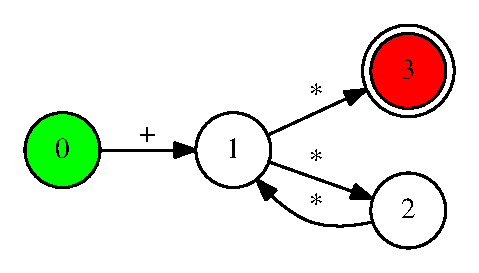
\includegraphics[width=120pt]{picts/InputGraph.eps}
 		\item Спецификация
 		\\
 		\begin{verbatim}
 		PLUS : "+"
 		POW : "**"
 		MULT: "*"
 		\end{verbatim}
		\item Результат токенизации
    \\
    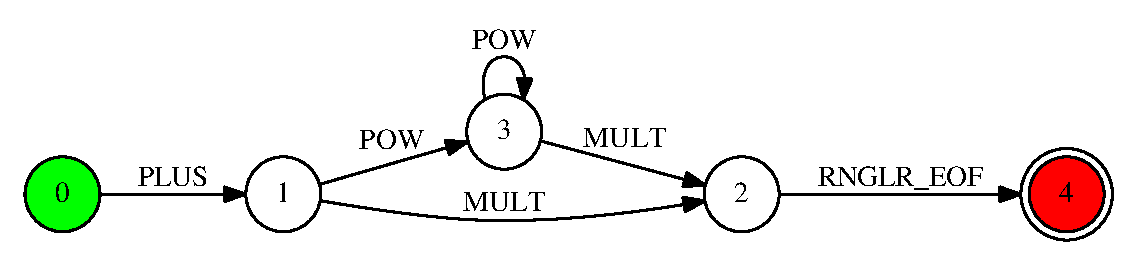
\includegraphics[width=250pt]{picts/TestInterpretParser.eps}

	\end{itemize}
\end{frame}

\begin{frame}[fragile]
	\transwipe[direction=90]
	\frametitle{Регулярная аппроксимация: строковые операции}
	\begin{itemize}
		\item \verb|result = replace(src_str, old, new)|		
 		\item \verb|src_str|: 
 		\\
    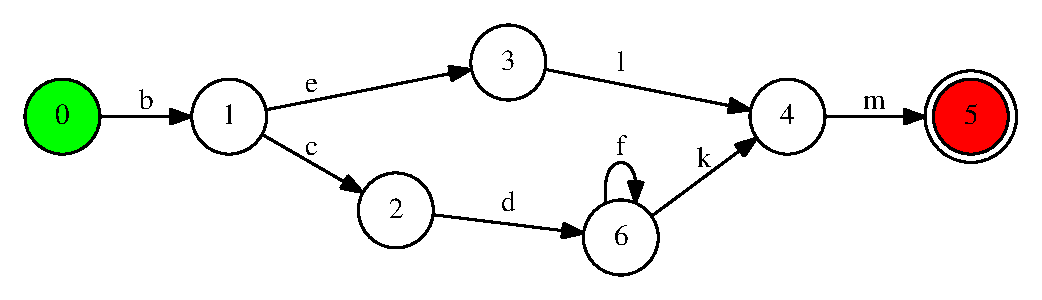
\includegraphics[width=220pt]{picts/fsa1.eps}
    \item
    \begin{tabular}[t t t t]{l l l l }
    %\begin{itemize}
     \verb|old|:
      &
       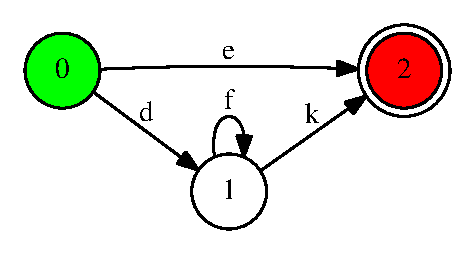
\includegraphics[width=80pt]{picts/fsa2.eps}
    %\end{itemize} 
 		&
 		%\begin{itemize}
     \verb|new|:
        &
          \includegraphics[width=50pt]{picts/fsa3.eps}
    %\end{itemize}

    \end{tabular}
		\item \verb|result|:
    \\
    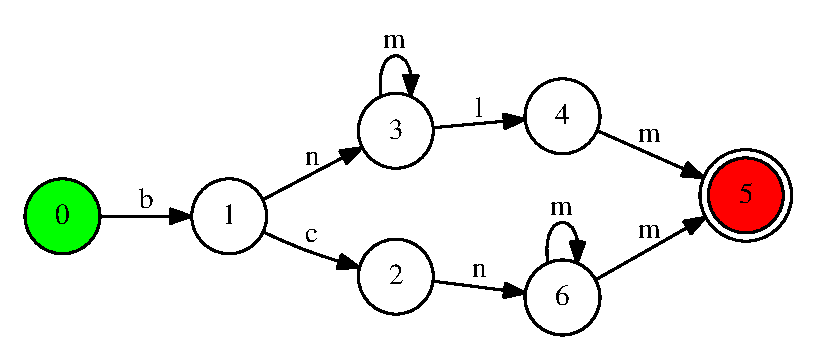
\includegraphics[width=220pt]{picts/replace_example.eps}

	\end{itemize}
\end{frame}

\begin{frame}
	\transwipe[direction=90]
	\frametitle{Литература}
	\begin{itemize}
		\item RNGLR: \emph{Scott E., Johnstone A.} Right Nulled GLR Parsers.
		\item Alvor: \emph{Aivar Annamaa, Andrey Breslav, Jevgeni Kabanov, and Varmo Vene}. 2010. An Interactive Tool for Analyzing Embedded SQL Queries.
		\item JSA: \emph{Aske Simon Christensen, Anders Møller, and Michael I. Schwartzbach}. Precise Analysis of String Expressions.
    \item PHPSA: \emph{Yasuhiko Minamide}. 2005. Static approximation of dynamically generated Web pages.
    \item Abstract parsing: \emph{Kyung-Goo Doh, Hyunha Kim, and David A. Schmidt.} 2011. Abstract LR-parsing.
    \item Построение регулярной апроксимации: \emph{Fang Yu, Muath Alkhalaf, Tevfik Bultan, and Oscar H. Ibarra.} 2014. Automata-based symbolic string analysis for vulnerability detection.
	\end{itemize}
\end{frame}

\begin{frame}
	\transwipe[direction=90]
	\frametitle{Литература}
	\begin{itemize}
    \item О инструментах для работы со встроенными языками
      \begin{itemize}
        \item \emph{Hung Viet Nguyen,Christian Kästner, Tien N. Nguyen.}Varis: IDE Support for Embedded Client Code in PHP Web Applications.
        \item \emph{Zachary Smith.} 2011. Development of tools to manage embedded SQL.
      \end{itemize}
    \item Зачем могут быть нужны трансформации
      \begin{itemize}
        \item \emph{Martin Mariusz Lester.} 2013. Position paper: the science of boxing.
        \item \emph{Martin Lester, Luke Ong, Max Schaefer.} Information Flow Analysis for a Dynamically Typed Functional Language with Staged Metaprogramming.
      \end{itemize}
	\end{itemize}
\end{frame}

\end{document}
